\begin{comment}
\section{Non-Dimensional Simulations}
To run simulations in Non-Dimensionaly we have to find the non dimensional parameters for our problem.
We use Buckingham $\pi$ method to find out number of non dimensional parameters.
\begin{table}[H]
\centering
\begin{tabular}{||c c c c c c c c c c||}
 \hline
 Dimensional Variables & $\rho_L$ & $\rho_g$ & $\mu_L$ & $\mu_g$ & $\sigma_{Lg}$ & $L_b$ & $D_o$ & $H_o$ & $g$ \\
 \hline\hline
 M & 1 & 1 & 1 & 1 & 1 & 0 & 0 & 0 & 0 \\
 \hline
 L & -3 & -3 & -1 & -1 & 0 & 1 & 1 & 1 & 1\\
 \hline
 T & 0 & 0 & -1 & -1& -2 & 0 & 0 & 0 & -2 \\
 \hline
\end{tabular}
\caption{Dimensional matrix to determine non-dimensional groups}
\end{table}

Rank of the matrix = 3 \\

Number of independent non-dimensional parameters = 9-3 = 6 \\
\subsection{Domain}
\begin{figure}[H]
 \centering
 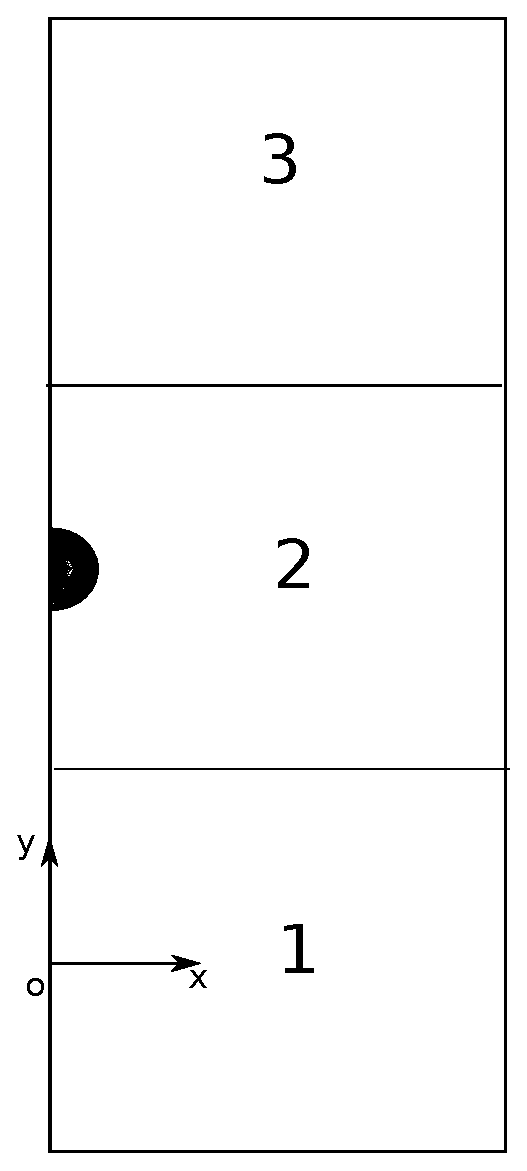
\includegraphics[scale=0.2]{domain}
 \caption{Domain for non-dimensional simulation}
\end{figure}

\subsection{Input to solver}
\begin{table}[H]
\centering
\begin{tabular}{||c c c||}
\hline
 Parameter & Remark & Value  \\ 
 \hline\hline
 Re & Reynolds number & 2521.285386 \\
\hline
 We & Weber number of Liquid-gas & 29.43 \\
 \hline
 $H_k$ & $\frac{H_o}{D_o}$ &  12.00\\
 \hline
 $L_k$ & $\frac{L_o}{D_o}$ &  2 \\
 \hline
 $\rho_k$ & $\frac{\rho_g}{\rho_L}$ & $2 X 10^{-3}$  \\ 
 \hline
 $\mu_k$ & $\frac{\mu_g}{\mu_L}$ & $2 X 10^{-2}$ \\
 \hline
 \end{tabular}
  \caption{Input for a multiphase solver in non-dimensional simulation}
 \end{table}
 
\subsection{Initial Condition}
The initial condition here is different from the dimensional simulation and compensates the differences in the governing
equations in both the simulations.
\begin{equation}
 x^2+(y+(H_k-0.5L_k))^2=0.25  %this equation is altered here from simulation there the axes are inverted
\end{equation}

\subsection{Boundary Conditions}
\begin{table}[H]
\centering
\begin{tabular}{||c c c c c||}
\hline
 Box ID & left & bottom & right & top  \\ 
 \hline\hline
 1 & free slip & no-slip, SCA = $150^o$ & no-slip & no-slip  \\ 
 \hline
 2 & - & no-slip, SCA = $150^o$ & no-slip & no-slip  \\ 
 \hline
 3 & - & no-slip, SCA = $150^o$ & no-slip & no-slip  \\ 
 \hline
\end{tabular}
 \caption{Boundary conditions for domain}
\end{table}
\end{comment}

\begin{comment}
\section{Dimensional and Non-Dimensional Simulations}

The problem has a initial condition for interface of the droplet at a height $H_o$ from the bottom of the domain. At a time step of 21
and equilavent dimensional time of 0.0749, it can be seen that both dimensional and non-dimensional simulation interface overlaps
each other (See Fig 5.1).
\begin{figure}[H]
 \centering
 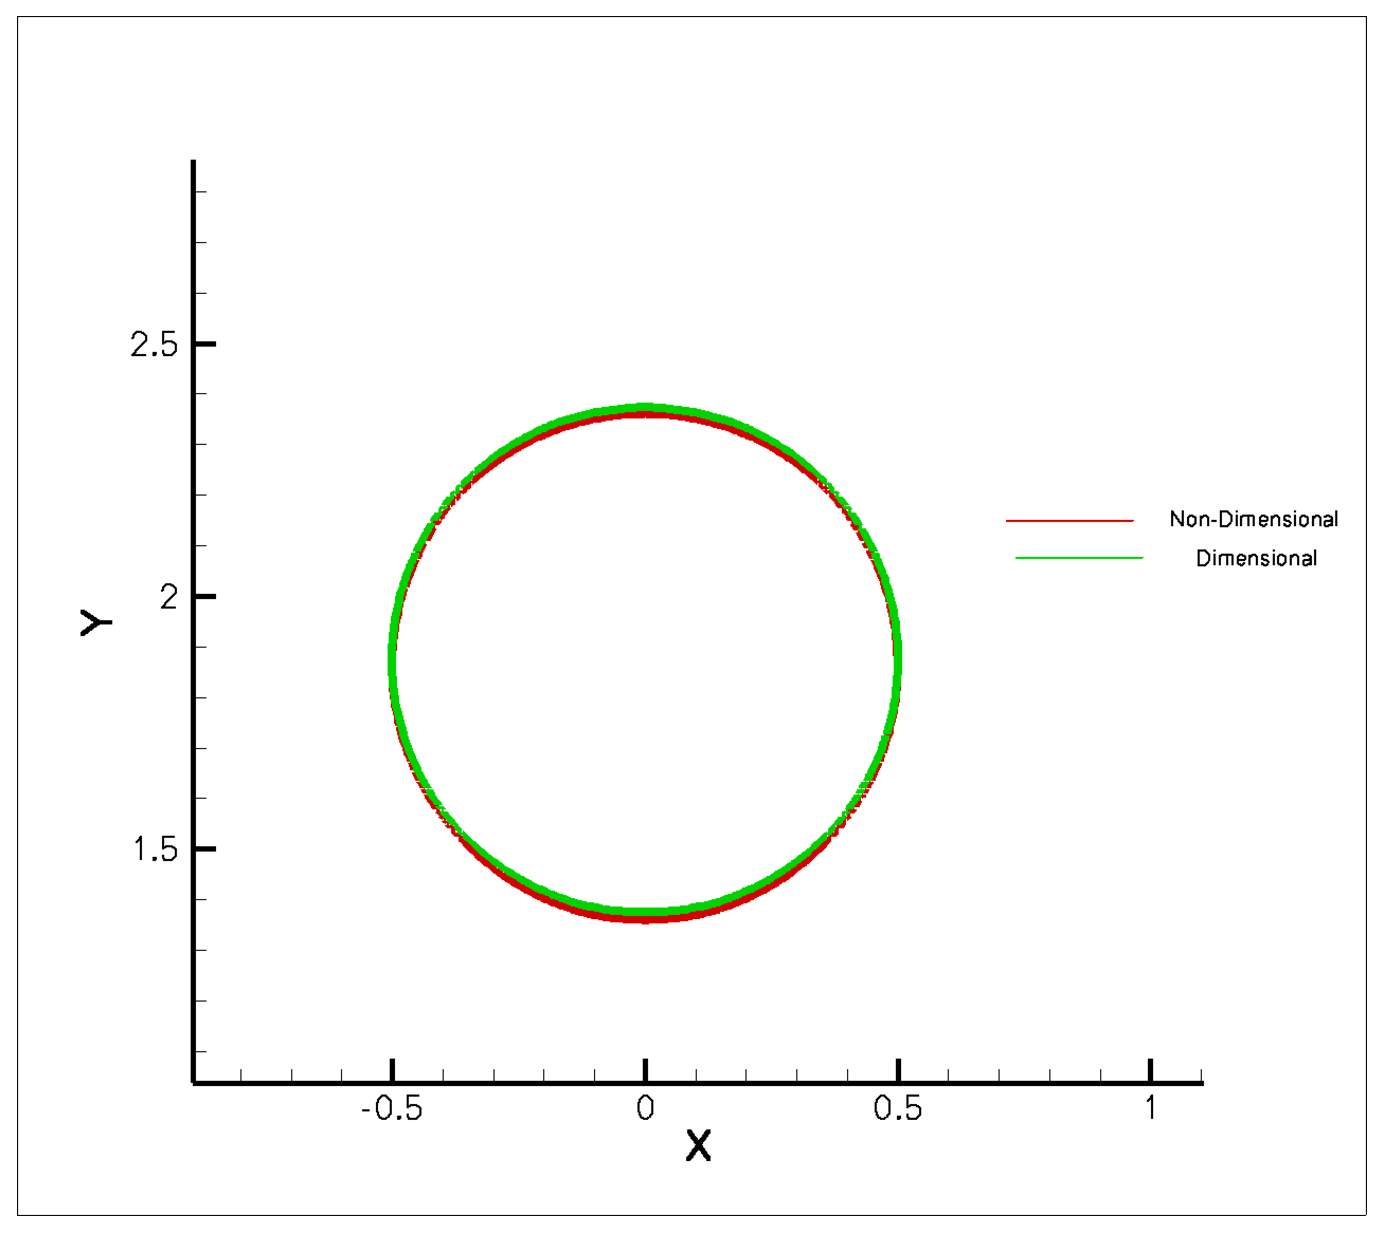
\includegraphics[scale=0.4]{tec21.eps}
 \caption[Comparison of dimensional and non-dimensional simulation]{Interface of droplet at equilavent times $t_{ND}$=21 and $t_D$=0.0749}
\end{figure}

\begin{figure}[H]
 \centering
 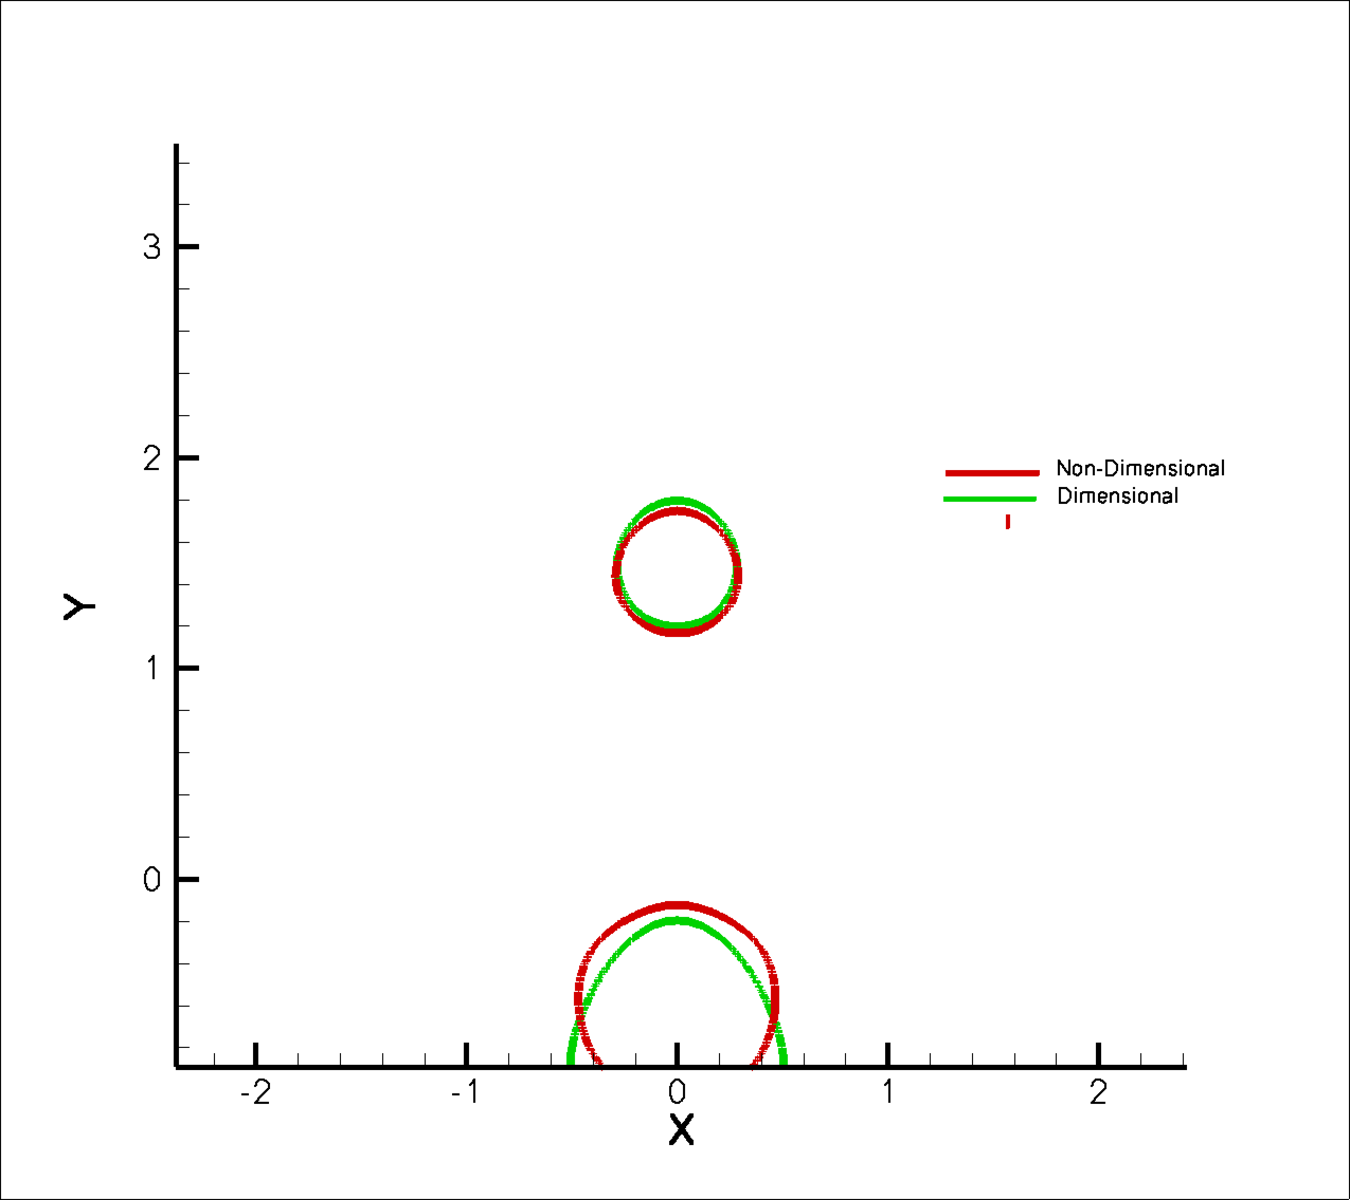
\includegraphics[scale=0.5]{tec48.ps}
 \caption[Comparison of dimensional and non-dimensional simulation]{Interface of droplet at equilavent times $t_{ND}$=48 and $t_D$=0.1712}
\end{figure}
For some time steps after the impact ($t_ND=48$, $t_D=0.1712$) it can be seen that the results are almost same, the minute differences
can be from the small time step difference or grid dependence.
\section{Effect of Boundary conditions}
\begin{figure}[H]
 \centering
 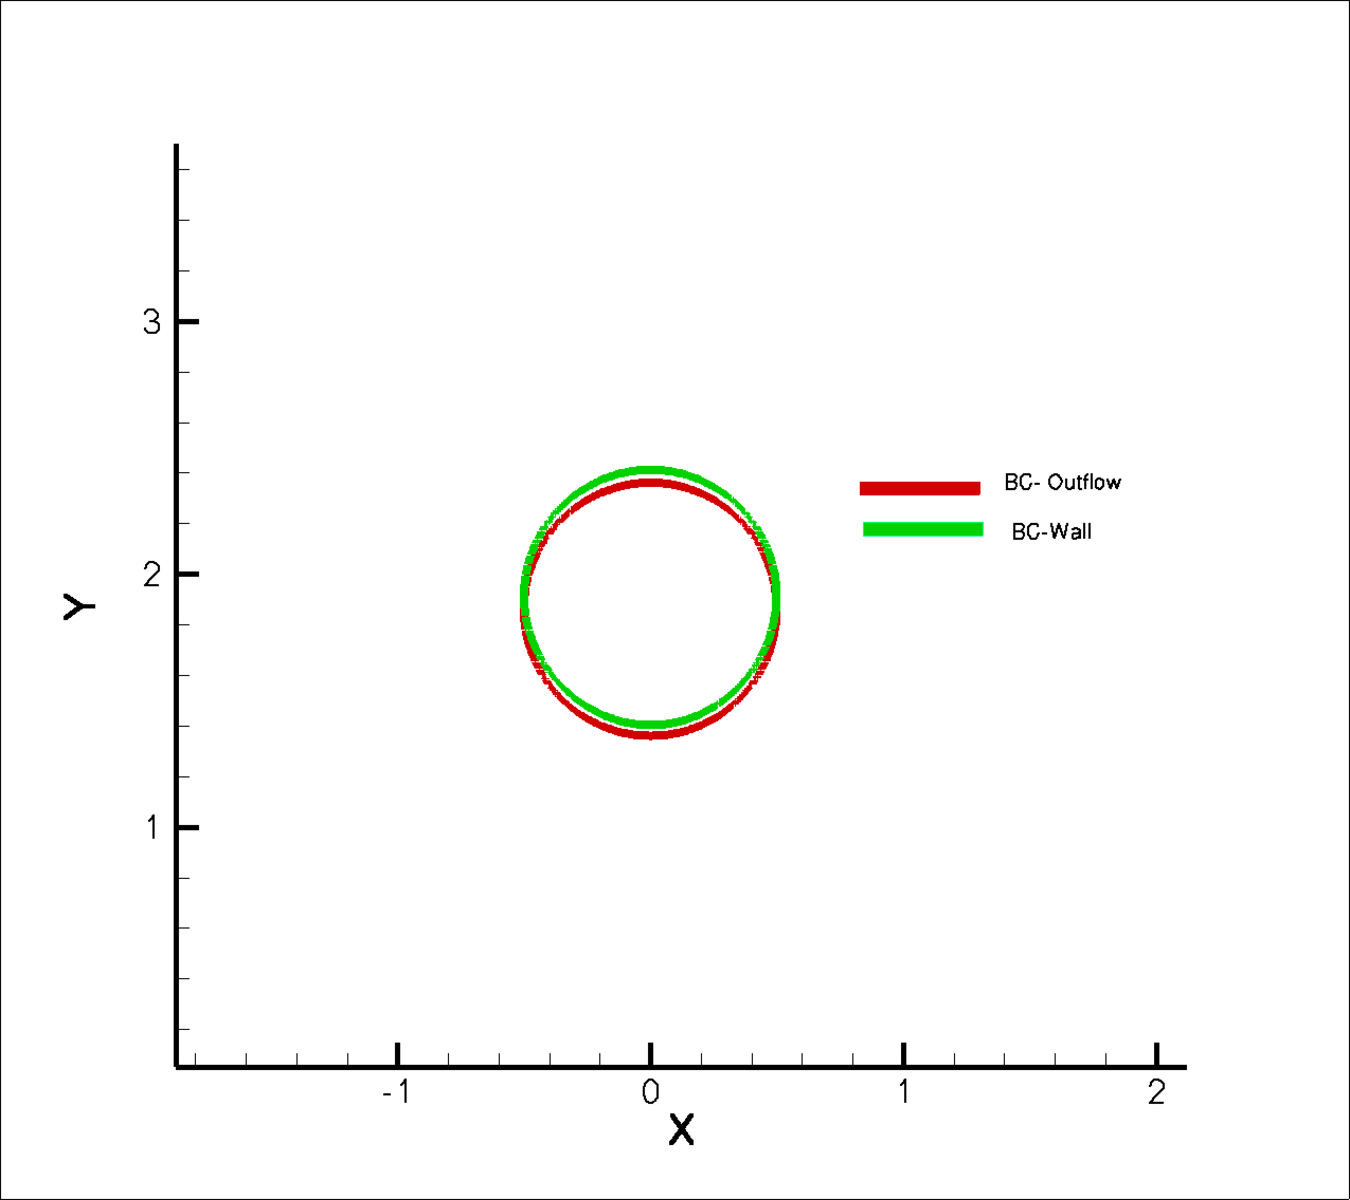
\includegraphics[scale=0.5]{tec-BC-21.ps}
 \caption[Effect of boundary conditions]{Interface of droplet at equilavent times $t_{ND}$=21 for slip wall conditions and outflow  at boundary }
\end{figure}
The boundary conditions did not affected the droplet motion initally as it can be seen from figure 5.3 but large variations can be seen
after the impact, the boundary condition on the boundaries of domain do have a impact on the results if the domain is of the order of size 
10 times the droplet diameter.
\begin{figure}[H]
 \centering
 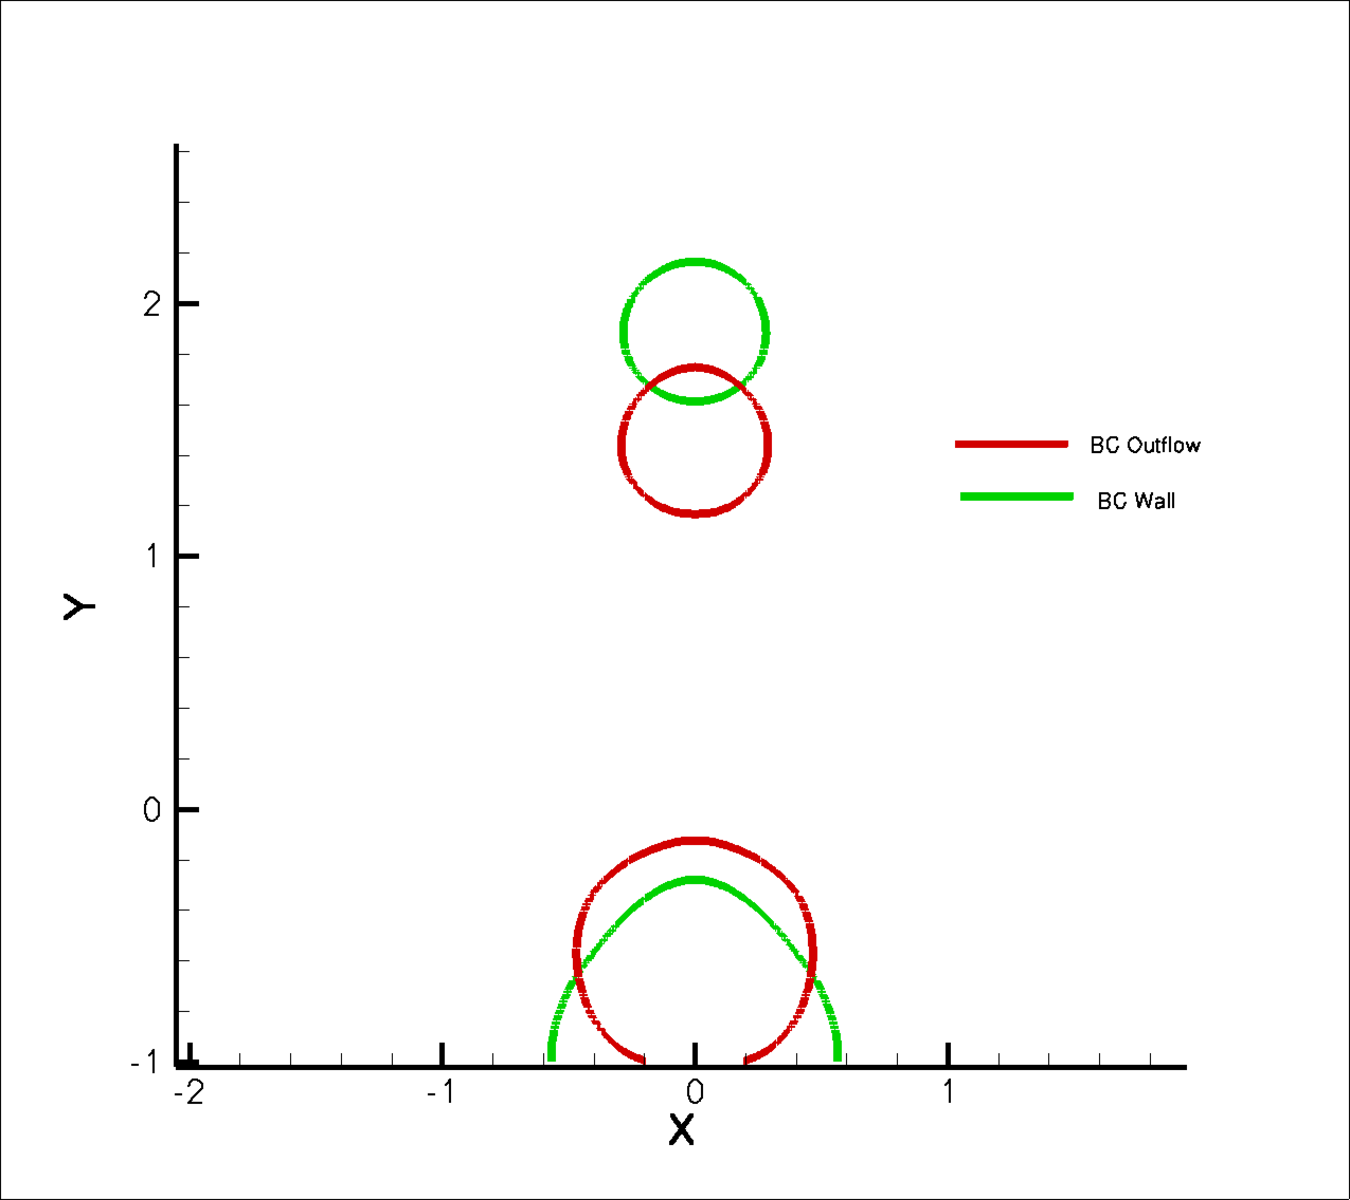
\includegraphics[scale=0.5]{tec-BC-48.ps}
  \caption[Effect of boundary conditions]{Interface of droplet at equilavent times $t_{ND}$=48 for slip wall conditions and outflow  at boundary }
\end{figure}
It is concluded that the domain size should be increased enough so that the influence of boundaries should be minimum on the dynamics
of droplet impact.
\section{Effect of domain shape}
\begin{figure}[H]
 \centering
 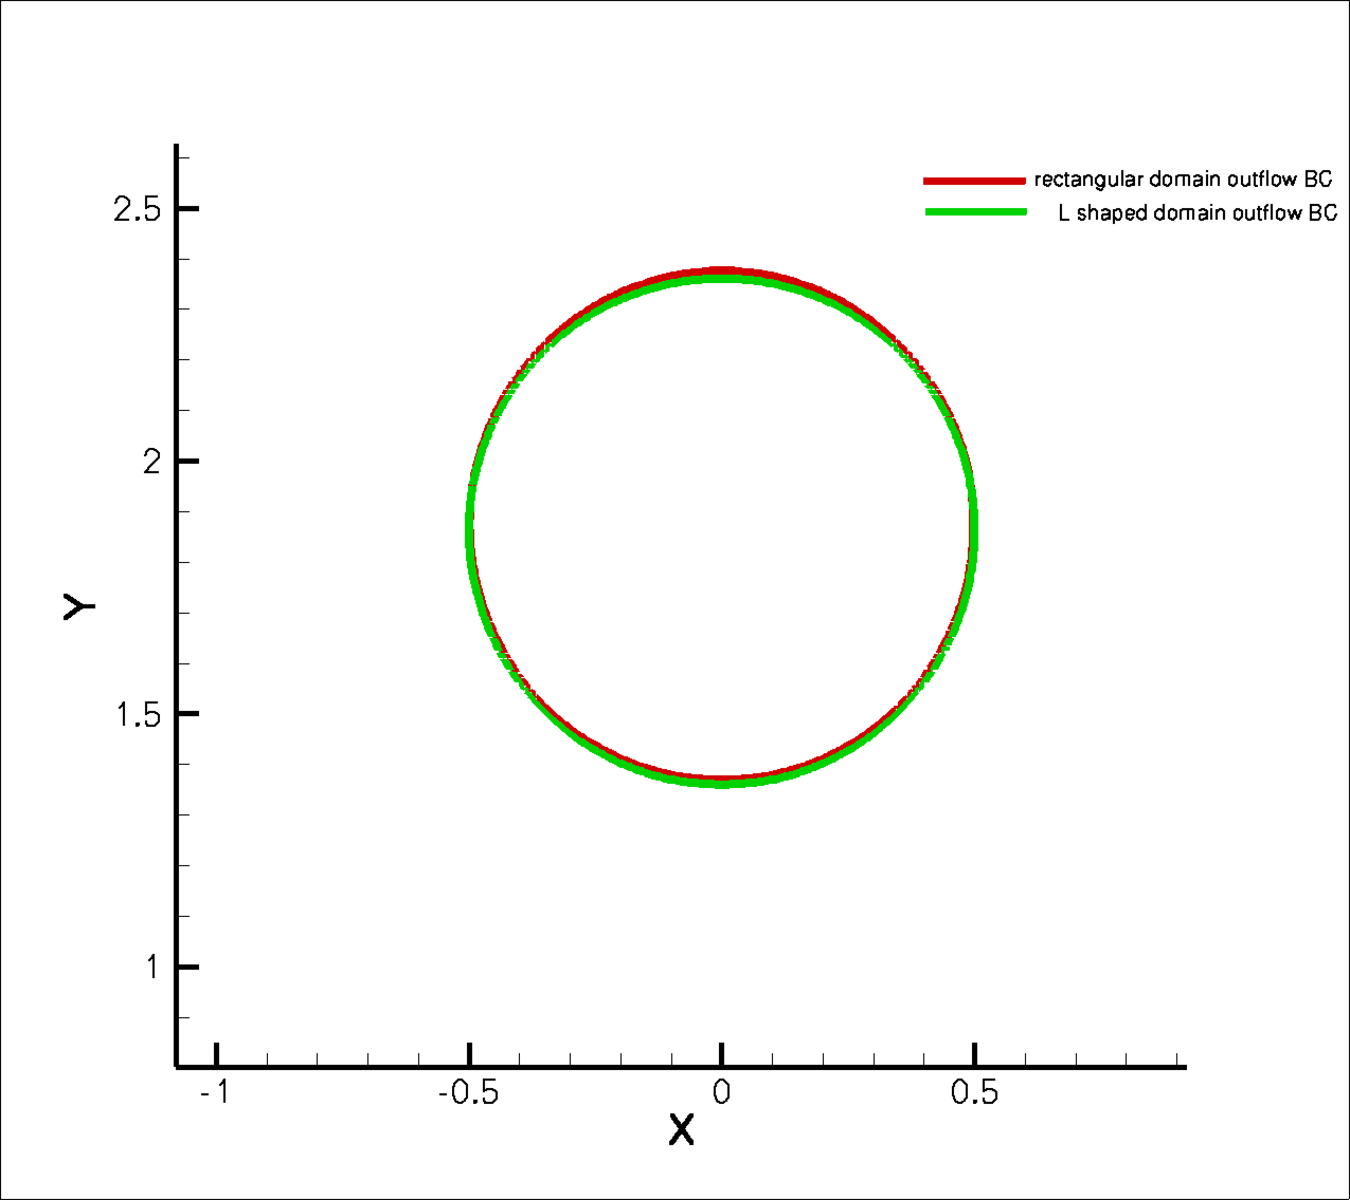
\includegraphics[scale=0.5]{tec-domain-21.ps}
 \caption[Effect of domain shape]{Interface of droplet at equilavent times $t_{ND}$=21 for rectangular domain and L shaped domain }
\end{figure}
The domain shape didn't affected the motion initially but have a great influence on the dynamics after the impact,
\begin{figure}[H]
 \centering
 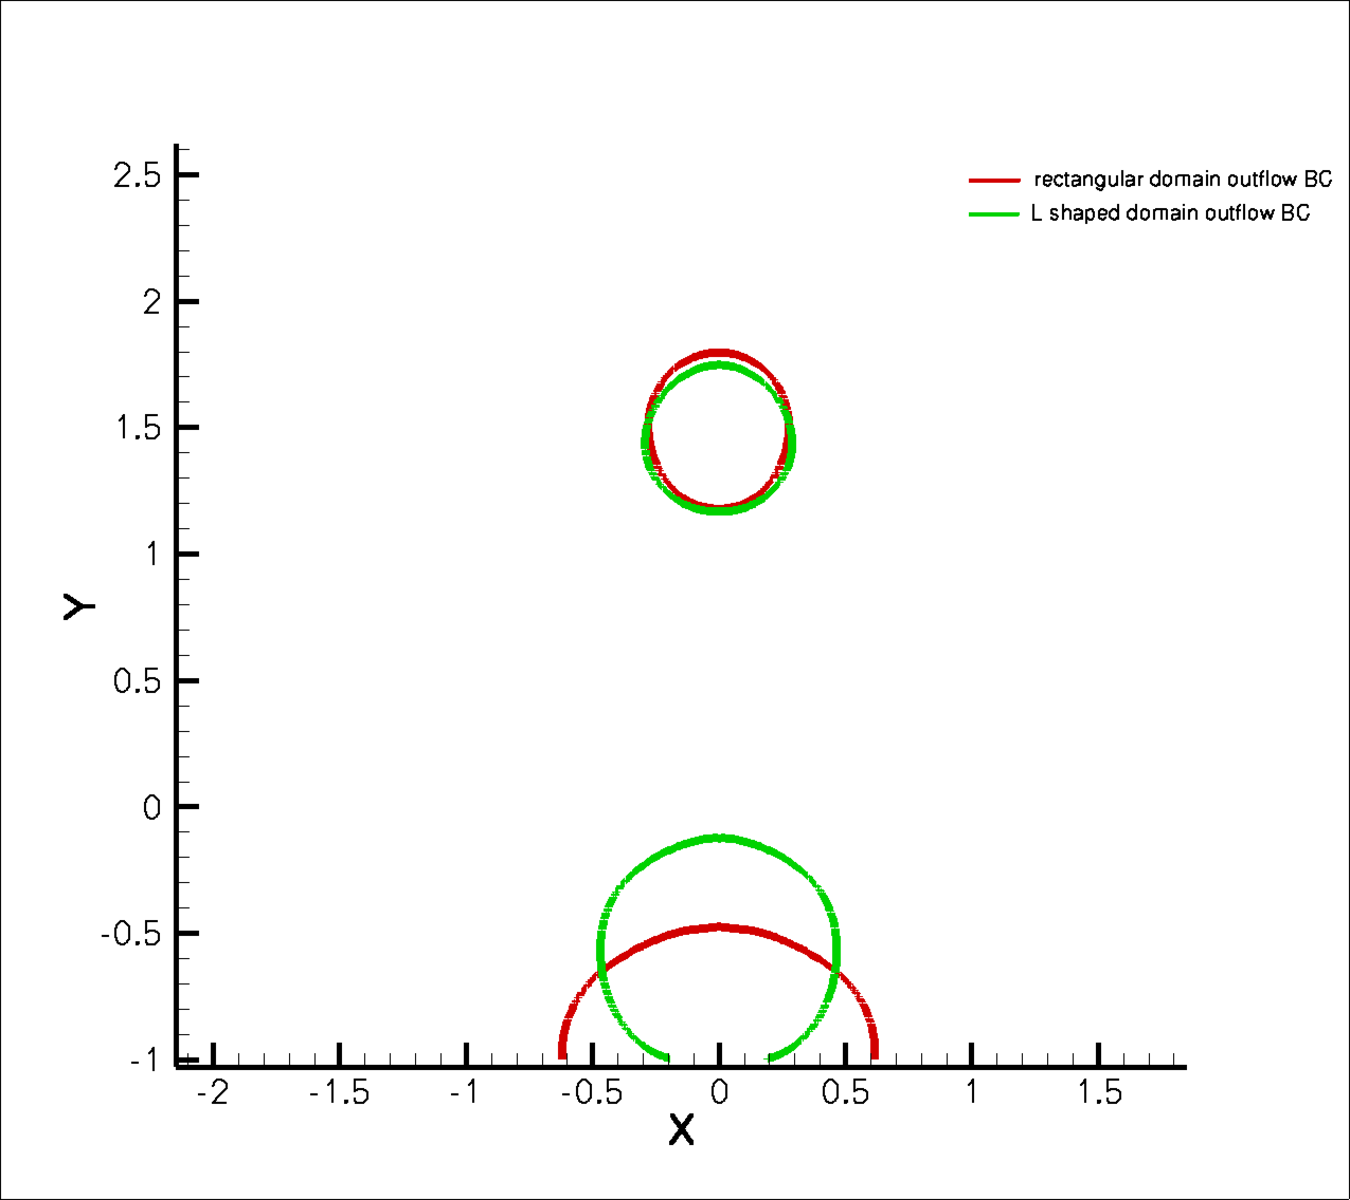
\includegraphics[scale=0.5]{tec-domain-48.ps}
  \caption[Effect of domain shape]{Interface of droplet at equilavent times $t_{ND}$=48 for rectangular domain and L shaped domain }
\end{figure}

It is therefore needed to have a shape which should not affect the droplet motion and impact.
\end{comment}